\section{Objetivo}

%Somos o banco X e vamos decidir se emprestamos ou não para o cliente Y (no nosso caso para a Positivo Informática S/A)
Por meio de uma análise detalhada e consolidada dos indicadores da empresa \nomeCompletoPositivo{}, define-se o risco de crédito (empréstimo) a mencionada empresa por parte do \emph{\nomeDoBanco{}}. Sendo assim, essa análise deve definir, seguindo métricas e métodos de controladoria gerencial, uma recomendação ao \emph{board} do banco para que possam tomar uma decisão referente ao mesmo.

\section{Risco de Crédito}

O \nomeDoBanco{} preza pelo respeito, ética, transparência e normas vigentes no sistema Bancário Brasileiro, inclusive com atenção as normas previstas na convenção da Basileia, já abrangendo a de número III.
Apenas para contextualizar de forma resumida e rápida, em 1988, o CBS divulgou o primeiro Acordo de Capital da Basileia, apresentado como Internacional Convergence of Capital Measurement and Capital Standards. O objetivo era criar as exigências mínimas de capital para todas instituições financeiras como forma de fazer frente ao risco de crédito.
Mesmo com a adoção das metodologias impostas pelo acordo de Basileia ainda aconteceram grandes desastres na economia mundial, como em 2007 e 2008. Essa crise em especial demonstrou que os acordos anteriores previstos em Basileia foram insuficientes para coibir a alavancagem abusiva dos bancos, a qual aliada à baixa qualidade do capital e à baixa margem de liquidez compunham o cenário de fragilidade do sistema bancário Americano e Internacional. Assim, como parte de um movimento contínuo de aprimoramento da estrutura prudencial aplicável às instituições financeiras, o Comitê de Basileia divulgou em dezembro de 2010 os normativos: Basel III, com três pilares a serem respeitados pelas instituições financeiras:

\begin{itemize}
\item Pilar 1: requerimentos de capital para risco de crédito, mercado e operacional;
\item Pilar 2: revisão pela supervisão do processo de avaliação da adequação de capital dos bancos;
\item Pilar 3: disciplina de mercado.
\end{itemize}

O Risco de Credito é sempre baseado em uma tomada de decisão com um certo nível de incerteza, seja qual for a modalidade de Credito adotada pela instituição. O Credor tem a obrigação de estimar a probabilidade de que essa  perda ocorra.
A estimativa desse Risco e “calculado” em função das características do cliente, no nosso caso a Positivo, utilizando modelos de \emph{Credit Scoring}.
No tocante ao nosso Cliente deve-se quantificar o “Risco Cliente” e a Operação desejada, pois grupos societários grandes como a Positivo diversificam seus investimentos em oportunidades que nem sempre são mensuráveis ou palpáveis no momento da concessão do credito.
O fundamento básico do nosso plano de Scoring será simples: Devemos analisar o Patrimonio do nosso cliente,o total de operações no mercado(Via BACEN), a quantidade de protestos ativos em cada CNPJ da organização. Com auxilio de um \emph{Bureau de Crédito} agregamos todos estes fatores num processo quantitativo, gerando desta forma , bem resumidamente, um Escore de credito, que normalmente e classificado de AA, A, B,C, ... H. Importante ressaltar que este Escore recebido pelos nossos clientes ‘e “Recalculado” periodicamente, por ocasião dos novos balancetes ou balancos, mudança na politica monetária e, também, por novos ativos adquiridos pelo Cliente.

\textcolor{blue}{A FAZER GRÁFICOS/PLANILHAS (KLEBER)}

\section{Histórico}
A Positivo Tecnologia nasceu do Grupo Positivo, que é o maior grupo do segmento de educação no Brasil. Fundado em 1972, a partir da criação de uma escola e de uma gráfica, o Grupo Positivo possui atualmente empresas líderes nos três segmentos em que atua: educacional, gráfico-editorial e tecnologia. A partir do grande sucesso de sua inovadora metodologia de ensino desenvolvida, aprimorada e sistematizada pelos conceituados professores fundadores do grupo, a rede de escolas próprias foi ampliada para os demais níveis educacionais e, em 1979, o grupo iniciou a venda de livros e serviços a outras escolas em todo Brasil.

Em 1989, os mesmos empreendedores do grupo iniciaram a produção de computadores pessoais, criando assim a Positivo Informática. Inicialmente, este ramo do grupo focou apenas na produção e comercialização de computadores para escolas clientes do Grupo Positivo em todo o Brasil. Atualmente, no ramo de tecnologia, a empresa produz computadores, laptops, tablets, smartphones, celulares e, mais recentemente, dispositivos de telemedicina. 

A semente original do grupo ainda se mantém, o grupo conta com cerca de 27 mil alunos em suas unidades próprias (Escolas Positivo, Curso Positivo e Universidade Positivo), além de ter atendido a aproximadamente 10 milhões de alunos com seus produtos e serviços desde sua fundação. Os Portais Educacionais do Grupo Positivo estão presentes em cerca de 11,0 mil escolas. Além disso, a Posigraf é a primeira gráfica Carbono Zero do país. O Grupo Positivo conta atualmente com mais de 9,0 mil colaboradores.

\section{Perfil Corporativo}

\begin{figure}[h]
\begin{centering}
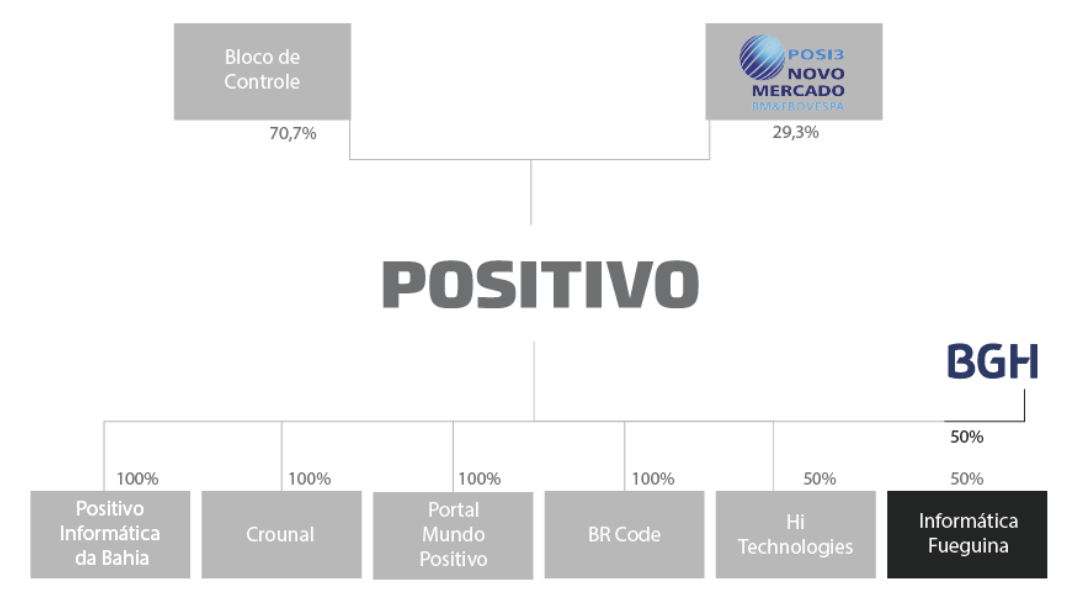
\includegraphics[width=1.0\textwidth]{Img/Corporativo}
\caption{Figura que demonstra o domínio e capital social da \nomeCompletoPositivo{}.}
\par\end{centering}
\end{figure}

Em 2016, a Positivo Tecnologia foi uma das maiores fabricantes de computadores no Brasil, respondendo por 15,3\% do número total de computadores vendidos no mercado brasileiro, de acordo com a IDC. No mesmo período, obtiveram uma participação de 19,9\% do mercado de varejo. Uma parcela substancial da produção de computadores é vendida através de grandes redes de varejo, com as quais o grupo mantém sólido relacionamento comercial, em função principalmente dos preços competitivos, do reconhecimento da marca e assistência técnica.

Adicionalmente, a companhia atua no mercado argentino por meio da marca \nomePositivoAr{}, fruto de uma joint venture com um parceiro local. Em 2015, os computadores \nomePositivoAr{} atingiram uma participação de 9,5\%, segundo a IDC.

No Brasil, a Positivo Tecnologia oferece uma linha completa de dispositivos, incluindo computadores de mesa (desktops e all-in-ones), computadores portáteis (notebooks e netbooks) e tablets, que são produzidos em Manaus (AM). Em 2012, a Companhia ingressou no mercado de telefones celulares, com a oferta de smartphones e messaging phones.

\begin{figure}[h]
\begin{centering}
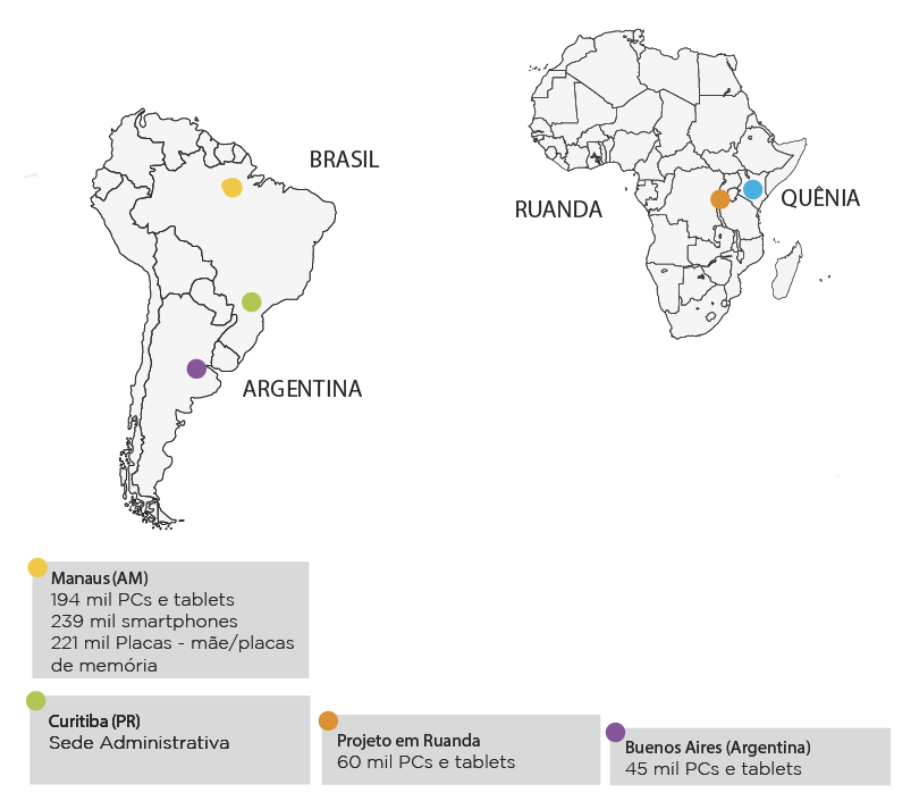
\includegraphics[width=1.0\textwidth]{Img/PositivoMundo}
\caption{Operações da \nomePositivo{} a nível mundial, bastante expressiva na América Latina e observa-se também sítios na África.}
\par\end{centering}
\end{figure}

Além disso, para atendimento e suporte aos milhões de consumidores finais, empresas e órgãos do governo, conta com uma ampla e capacitada rede de assistências técnicas cobrindo a totalidade do território nacional, e com a CRP - Central de Relacionamento Positivo, que registrou em média, 2,9 mil contatos diários em 2016. Grande parte destes contatos se refere a questões básicas sobre uso do computador, sistema operacional ou problemas com conexões, uma vez que muitos dos clientes estão adquirindo seu computador pela primeira vez.

Parcela menor da receita da Companhia provém do Segmento de Tecnologia Educacional, no qual acredita ser líder absoluto no País. A Companhia oferece soluções de infraestrutura e gestão, aplicativos e plataformas educacionais, portais de educação, além de formação de professores e acompanhamento pedagógico. Os portais têm mais de 1,2 milhões de usuários ativos, com modelo de receita recorrente mensal. 

As soluções educacionais da Positivo Tecnologia estão presentes em mais de 14 mil escolas e são exportadas para mais de 40 países. Dentre os principais produtos estão mesas educacionais, dispositivos móveis, lousas interativas, dispositivos de armazenamento e recarga, projetores, acess point, e sistema de gerenciamento de aulas. A Companhia é também distribuidor exclusivo no Brasil de empresas líderes no desenvolvimento e distribuição de software educacional, bem como distribui produtos da LEGO\texttrademark Education no território nacional.

Em 2016, a Companhia ingressou no mercado de tecnologia médica por meio da aquisição de 50\% do capital social da Hi Technologies S.A., empresa com forte foco em P\&D para a oferta de produtos inovadores em saúde.
